\documentclass[tikz, border = 10pt]{standalone}

\usepackage{newpxtext,newpxmath}   % /upbeta
%\usepackage{fouriernc}            % /otherbeta
\usepackage{amsmath}
\renewcommand{\familydefault}{\sfdefault}
\usepackage{mathastext}

\usetikzlibrary{positioning, quotes, calc, math, arrows.meta, bending, shapes, backgrounds}

\tikzset{
every edge quotes/.style = {fill = white},
every node/.style = {scale = 1.1},
manifest/.style = {rectangle, draw, thin, inner sep = 3pt, minimum width = 1cm,
   minimum height = .85cm, align = center},
latent/.style = {ellipse, draw, thin, inner sep = 3pt, minimum width = 1cm,
   minimum height = .85cm},
residual1/.style = {circle, draw, thin, minimum size = 5mm, inner sep = 1pt},
residual2/.style = {rectangle, minimum width = 0.5pt, minimum height = 1.5mm,
   inner sep = 0pt, outer sep = 0mm},
regression/.style = {-{Stealth[length = 1.5mm]}, thin, shorten > = 1pt, 
   inner sep = 1.5pt, outer sep = 0mm},
covariance/.style={{Stealth[length = 1.5mm]}-{Stealth[length = 1.5mm]}, thin,
   shorten > = 1pt, shorten < = 1pt, inner sep = 1.5pt},
variance/.style={{Stealth[length = 1mm]}-{Stealth[length = 1mm]}, thin,
   shorten > = 1pt, shorten < = 1pt, inner sep = 1pt},
interaction/.style = {-{Stealth[sep = 1pt, length = 1.5mm] . Circle[length = 4pt]},
   thin, shorten > = -2pt},
constant/.style = {draw, thin, inner sep = 1pt, regular polygon,
   regular polygon sides = 3, minimum size = 5mm},
group/.style = {rectangle, inner sep = 2pt, minimum width = 15mm, minimum height = 5mm, 
   align = center}
}

\begin{document}
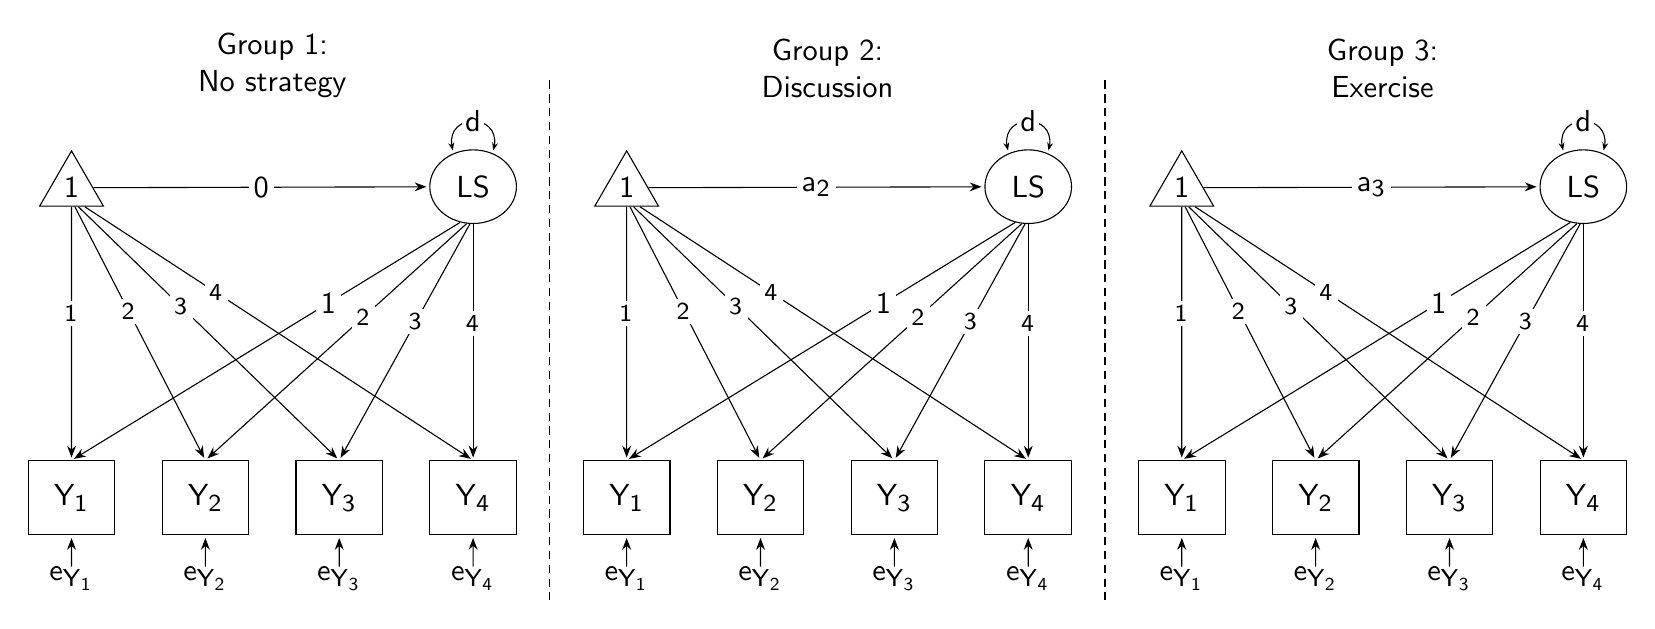
\begin{tikzpicture}

%% Dependents and their residuals
\foreach \i [remember = \x as \lastx (initially 0)] in {1,...,12}{
   \tikzmath{\labnum = int(mod(\i - 1, 4) + 1);} 
   \node [manifest] (y\i) at (\lastx, 0) {Y$_{\labnum}$};
   \node [residual2] (e\i) [below = 4mm of y\i] {e$_{Y_\labnum}$};
   \path [regression] (e\i) edge (y\i);  
   \ifnum \labnum = 4  \def\d{0.85} \else \def\d{0.6} \fi   
   \tikzmath{\x = \lastx + \d + 1.1;} 
}

%% Latent
\foreach \i/\j in {1/No strategy, 2/Discussion, 3/Exercise} {
   \tikzmath{\x = int(4*\i);}
   \node [latent] (latent\i) [above = 3cm of y\x] {LS};

   %% Latent variances
   \path [variance] (latent\i.120) edge ["d", bend left = 110, looseness = 3] (latent\i.60);

   %% Means
   \tikzmath{\x = int(\x - 3);}
   \node [constant] (const\i) [above = 3.22cm of y\x] {1};
   \path[regression] (const\i) edge ["\ifnum \i = 1 {0} \else {a$_\i$} \fi"] (latent\i);

   \foreach \b/\c/\d in {1/270/250, 2/280/260, 3/290/265, 4/305/270} {
      %% Intercepts
      \tikzmath{\e = int((\i - 1)*4 + \b);} 
      \path [regression] (const\i.\c) edge ["$\uptau_\b$", pos = 0.45 - 0.5/(4.5*(5-\b))] (y\e.90);

      %% Loadings
      \path[regression] (latent\i.\d) edge ["\ifnum \b = 1 {1} \else {$\uplambda_\b$} \fi", 
      pos = 0.45 - 0.5/(4.5*\b)] (y\e.90);
   }

   %% Groups
   \tikzmath{\xa = int(\x + 1);}
   \tikzmath{\xb = int(\x + 2;}
   \node [group] (gp\i) [above = 5cm of $(y\xa)!0.5!(y\xb)$] {Group \i:\\\j};
}  

%% Separators
\foreach \i in {4,8} {
   \tikzmath{\j = int(\i + 1);}
   \coordinate (M) at ($(y\i)!0.5!(y\j)$);
   \draw [style = densely dashed, thin] ($(M)!5.3cm!270:(y\i)$) -- ($(M)!1.3cm!90:(y\i)$);
}

\end{tikzpicture}
\end{document}